\documentclass[sigconf,nonacm]{acmart}

\setcopyright{none}
\settopmatter{printacmref=false}
\renewcommand\footnotetextcopyrightpermission[1]{}
\pagestyle{plain}

\usepackage{graphicx}
\usepackage{booktabs}
\usepackage{tabularx}
\usepackage{array}
\usepackage{tikz}
\usetikzlibrary{shapes,arrows.meta,positioning,fit,backgrounds,calc}
\usepackage{url}
\urlstyle{rm}

%% ── Colours ──────────────────────────────────────────────────────────────────
\definecolor{cred}   {RGB}{220, 80, 70}
\definecolor{cyellow}{RGB}{240,190, 50}
\definecolor{cblue}  {RGB}{ 70,120,200}
\definecolor{cgreen} {RGB}{ 60,170, 90}
\definecolor{corange}{RGB}{230,130, 40}
\definecolor{cgray}  {RGB}{100,100,100}
\definecolor{clightb}{RGB}{210,225,250}
\definecolor{clightg}{RGB}{210,240,215}
\definecolor{clighto}{RGB}{255,235,200}
\definecolor{clightr}{RGB}{255,215,210}

\title{Compensating Controls and Architecting for Cyber Resilience:\\
Bridging the Gap Between Compliance Requirements and Operational Reality}

\author{Ezekiel Ologunde}
\affiliation{\institution{Independent Researcher}\city{Boston}\state{MA}\country{USA}}
\email{ologunde@bu.edu}

\begin{abstract}
Organizations frequently encounter scenarios where recommended cybersecurity controls
are technically sound but operationally impracticable due to legacy system constraints,
financial limitations, or mission-critical availability requirements. This paper examines
the strategic role of compensating controls as deliberate architectural decisions rather
than compliance shortcuts, demonstrating how alternative security measures can provide
equivalent protection when primary controls prove infeasible. Through analysis of
real-world scenarios---particularly in operational technology and defense contractor
environments---we illustrate how network segmentation, enhanced monitoring, and identity
governance can substitute for incompatible endpoint detection solutions. Building upon
this foundation, the paper explores broader architectural concepts that enhance cyber
resilience, including defense-in-depth strategies, network isolation, recovery
engineering, and detection-focused investments. Drawing on recent regulatory developments
including the 2023 New York DFS cybersecurity regulation amendments, PCI DSS v4.0
compensating control frameworks, and contemporary OT security research, we demonstrate
that effective compensating controls require rigorous justification, measurable risk
reduction, and continuous reassessment. Our analysis reveals that cyber resilience is
not about achieving perfect prevention but about building systems capable of withstanding,
detecting, responding to, and recovering from inevitable adversarial activity.
\end{abstract}

\begin{CCSXML}
<ccs2012>
  <concept>
    <concept_id>10002978.10003029</concept_id>
    <concept_desc>Security and privacy~Systems security</concept_desc>
    <concept_significance>500</concept_significance>
  </concept>
  <concept>
    <concept_id>10002978.10003006</concept_id>
    <concept_desc>Security and privacy~Risk assessment</concept_desc>
    <concept_significance>500</concept_significance>
  </concept>
  <concept>
    <concept_id>10002978.10003022</concept_id>
    <concept_desc>Security and privacy~Security services</concept_desc>
    <concept_significance>300</concept_significance>
  </concept>
</ccs2012>
\end{CCSXML}

\ccsdesc[500]{Security and privacy~Systems security}
\ccsdesc[500]{Security and privacy~Risk assessment}
\ccsdesc[300]{Security and privacy~Security services}

\keywords{Compensating controls; cyber resilience; defense-in-depth; operational
technology security; CMMC compliance; network segmentation; detection and monitoring;
recovery engineering}

\begin{document}
\maketitle

%%──────────────────────────────────────────────────────────────────────────────
\section{Introduction}
%%──────────────────────────────────────────────────────────────────────────────

Organizations implementing cybersecurity programs routinely encounter a fundamental
tension: governance frameworks prescribe controls that are technically feasible in
theory but operationally impracticable in specific environments. This challenge
manifests acutely in sectors with legacy operational technology, resource-constrained
small businesses, and mission-critical systems where availability requirements preclude
certain security implementations. Frameworks such as NIST SP 800-53 and the
Cybersecurity Maturity Model Certification (CMMC) establish baseline security controls
without necessarily accounting for operational constraints, legacy system limitations,
or cost barriers that make literal compliance
infeasible~\cite{nist2020controls,dod2021cmmc}.

The challenge for CISOs and security architects is not merely achieving compliance
checkboxes but demonstrating \emph{why} required controls are not feasible while
proposing compensating controls that provide equivalent levels of protection. As recent
guidance emphasizes, compensating controls are not shortcuts or fallbacks but deliberate
choices---alternative ways to reduce exposure when the preferred control is not
practical~\cite{reach2024,fortinet2024}. When implemented with intent, clarity, and
rigorous documentation, compensating controls strengthen security posture rather than
weakening it~\cite{metricstream2024}.

Regulatory frameworks have evolved to explicitly accommodate compensating controls.
The New York Department of Financial Services' 2023 cybersecurity regulation amendments
permit CISO-approved compensating controls for specific requirements, provided they are
documented in writing and reviewed annually~\cite{koleyjessen2024}. PCI DSS version 4.0
includes comprehensive guidance on compensating control documentation, requiring
organizations to complete detailed worksheets addressing constraints, objectives,
identified risks, validation, and maintenance~\cite{techtarget2024}.

Beyond individual control substitutions, organizations must architect systems for cyber
resilience---the capacity to withstand, detect, respond to, and recover from adversarial
cyber activity. Modern cyber resilience frameworks assume that breaches are inevitable
and therefore emphasize system robustness, rapid detection, effective response, and swift
recovery rather than relying solely on preventive controls~\cite{zeronetworks2024,
guidehouse2023}.

%%──────────────────────────────────────────────────────────────────────────────
\section{Research Objectives}
%%──────────────────────────────────────────────────────────────────────────────

This paper addresses the following objectives:
\begin{enumerate}
  \item Articulate scenarios where recommended controls prove impracticable and justify
        the use of compensating controls.
  \item Provide structured guidance for designing, implementing, and documenting
        compensating controls.
  \item Analyze the advantages and limitations of compensating control strategies.
  \item Identify architectural concepts that enhance cyber resilience.
  \item Establish decision frameworks for selecting resilience concepts based on
        organizational context.
\end{enumerate}

%%──────────────────────────────────────────────────────────────────────────────
\section{Theoretical Foundation}
%%──────────────────────────────────────────────────────────────────────────────

\subsection{Compensating Controls: Definition}

NIST defines compensating security controls as ``management, operational, and technical
controls employed by an organization in lieu of recommended controls that provide
equivalent or comparable protection for an information system''~\cite{nistglossary2024}.
This establishes three critical requirements: compensating controls must be
(1)~alternative measures when primary controls cannot be implemented,
(2)~provide equivalent or comparable protection, and
(3)~be formally justified and documented.

\subsection{Regulatory Evolution}

The Payment Card Industry Data Security Standard (PCI DSS) pioneered formal compensating
control requirements in 2004, establishing that they give organizations alternatives when
security requirements cannot be met ``due to legitimate and documented technical or
business constraints''~\cite{techtarget2024,fortinet2024}. PCI DSS v4.0 requires
compensating control worksheets covering: documentation of constraints; definition of
objectives; assessment of additional risks; validation of effectiveness; and maintenance
procedures~\cite{techtarget2024}.

NIST SP 800-53 similarly acknowledges that organizations may employ compensating controls
when recommended baseline controls cannot be implemented due to legitimate constraints,
emphasizing that they must undergo risk assessment to verify adequate
protection~\cite{nist2020controls,specops2022}.

\subsection{The Detective vs.\ Preventive Principle}

An illustrative metaphor involves barn mice control: sealing every possible entry point
(preventive control) would be prohibitively expensive and still ineffective. Employing
barn cats (detective and reactive measure) provides cost-effective protection by detecting
and responding to threats after they manifest. This principle applies directly to
cybersecurity: forcing legacy systems to run modern EDR may be both costly and
unreliable, while compensating controls emphasizing detection, monitoring, and response
may provide more practical risk reduction~\cite{reach2024}.

\subsection{Cyber Resilience Framework}

NIST defines cyber resilience as the ability to anticipate, withstand, recover from, and
adapt to adverse conditions, stresses, attacks, or compromises on
systems~\cite{nist2021resilience}. This explicitly acknowledges that perfect prevention
is unattainable and that security architectures must incorporate detection, response, and
recovery capabilities.

Recent research demonstrates tangible benefits: organizations with strong resilience
reduce cyber incident impact by 40\%, with well-tested incident response strategies
containing breaches 54 days faster on average~\cite{zeronetworks2024}. The average
global cost of a data breach in 2024 reached \$4.88 million---a record 10\% increase
over the prior year~\cite{ibm2024breach}.

%%──────────────────────────────────────────────────────────────────────────────
\section{Scenario Analysis}
%%──────────────────────────────────────────────────────────────────────────────

\subsection{Legacy Operational Technology Systems}

Consider a small defense contractor operating legacy OT systems controlling
mission-critical manufacturing processes. These systems cannot support modern EDR
software without risking system crashes or unacceptable performance degradation. EDR
represents a recommended security control under frameworks like CMMC and NIST SP 800-53,
yet installing it may jeopardize availability---one of three core security objectives
alongside confidentiality and integrity~\cite{nist2020controls}. This presents a
dilemma: comply and risk operational failure, or forgo the control and risk audit
deficiencies.

\subsection{OT:ICEFALL and ICS Vulnerabilities}

The OT:ICEFALL disclosure of 56 vulnerabilities affecting thousands of OT devices from
ten major vendors highlighted that many systems remain ``insecure by design'' despite
certifications suggesting otherwise~\cite{claroty2024}. For ICS and SCADA environments
that cannot be patched or modernized without extensive operational disruptions,
traditional patching and EDR deployment are often infeasible. Proactively implementing
risk-informed policies in accordance with Zero Trust architecture can greatly reduce
the likelihood and mitigate risks posed by exploitation of known and unknown
vulnerabilities in OT environments~\cite{claroty2024,rockwell2024}.

\subsection{Financial and Resource Constraints}

Beyond technical limitations, financial and resource constraints create scenarios where
recommended controls prove impracticable. Third-party systems may not support required
security features like multi-factor authentication or comprehensive logging, necessitating
alternative approaches~\cite{fortinet2024,metricstream2024}.

%%──────────────────────────────────────────────────────────────────────────────
\section{Designing Effective Compensating Controls}
%%──────────────────────────────────────────────────────────────────────────────

\subsection{Documentation Requirements}

When organizations decide not to implement recommended controls, compensating controls
must address underlying risks in measurable ways. Best practices
require~\cite{fortinet2024,reach2024}:
\begin{enumerate}
  \item \textbf{Document Constraints}: Clearly articulate why the original control was
        not feasible.
  \item \textbf{Identify Threat Scenario}: Specify the threat the original control was
        meant to mitigate.
  \item \textbf{Demonstrate Equivalence}: Show how the alternative provides comparable
        risk reduction.
  \item \textbf{Define Objectives}: Clarify how the compensating control meets the
        original objectives.
  \item \textbf{Validate Effectiveness}: Verify through testing, simulation, or audit.
  \item \textbf{Establish Maintenance}: Define processes for ongoing monitoring and
        reassessment.
\end{enumerate}

\begin{table}[h]
\caption{Compensating Control Documentation Requirements.}
\label{tab:documentation}
\small
\begin{tabularx}{\columnwidth}{@{}p{2.2cm}X@{}}
\toprule
\textbf{Element} & \textbf{Description} \\
\midrule
Constraint         & Technical, operational, or financial limitation preventing
                     primary control \\
\addlinespace[3pt]
Original Objective & Security goal of the primary control \\
\addlinespace[3pt]
Compensating Ctrl  & Alternative measure being implemented \\
\addlinespace[3pt]
Risk Assessment    & Analysis showing equivalent protection \\
\addlinespace[3pt]
Validation Method  & Testing or audit approach \\
\addlinespace[3pt]
Review Schedule    & Frequency of reassessment (typically annual) \\
\bottomrule
\end{tabularx}
\end{table}

\subsection{Example: EDR Substitution in OT Environments}

For scenarios where EDR cannot operate on legacy OT systems, compensating controls
include: (1)~enhanced network segmentation isolating OT from corporate IT networks,
deploying DMZs, and restricting lateral movement; (2)~strengthened identity governance
enforcing least-privilege, MFA for all remote access, and privileged access management;
(3)~continuous monitoring via network-based IDS, SIEM collecting available logs, and
behavioral baselines; and (4)~vulnerability management via regular scans, comprehensive
asset inventories, and risk-scored patch prioritization. These measures cannot perfectly
replicate EDR's preventive value, but they meaningfully reduce likelihood of compromise
while maintaining system stability~\cite{kelley2023}.

%%
%% FIGURE 1 — Compensating Control Lifecycle
%%
%% Design: vertical flowchart with 5 steps, right-hand feedback loop.
%% Box width = 3.6 cm centred at x=0  →  spans −1.8 to +1.8 cm.
%% Feedback arrow: right offset at x = +2.4 cm (well within ~4.3 cm half-column).
%% Total figure width ≈ 2×2.4 = 4.8 cm  ✓  (column ≈ 8.6 cm)
%%
\begin{figure}[h]
\centering
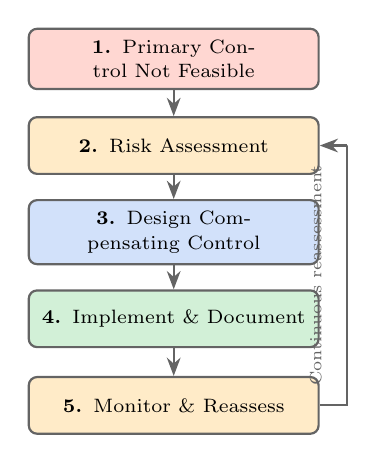
\begin{tikzpicture}[
  font=\fontsize{7pt}{9pt}\selectfont,
  >=Stealth,
  box/.style={
    rectangle, rounded corners=3pt,
    draw=cgray, thick,
    minimum width=3.6cm, minimum height=0.72cm,
    text centered, text width=3.4cm,
    inner sep=4pt
  },
  arr/.style={-{Stealth}, thick, cgray}
]
  %% ── Step nodes (spaced 1.1 cm apart) ────────────────────────────────────
  \node[box, fill=clightr] (s1) at (0, 0.00) {\textbf{1.} Primary Control Not Feasible};
  \node[box, fill=clighto] (s2) at (0,-1.10) {\textbf{2.} Risk Assessment};
  \node[box, fill=clightb] (s3) at (0,-2.20) {\textbf{3.} Design Compensating Control};
  \node[box, fill=clightg] (s4) at (0,-3.30) {\textbf{4.} Implement \& Document};
  \node[box, fill=clighto] (s5) at (0,-4.40) {\textbf{5.} Monitor \& Reassess};

  %% ── Down arrows ──────────────────────────────────────────────────────────
  \draw[arr] (s1.south) -- (s2.north);
  \draw[arr] (s2.south) -- (s3.north);
  \draw[arr] (s3.south) -- (s4.north);
  \draw[arr] (s4.south) -- (s5.north);

  %% ── Feedback loop: right side, from s5 back up to s2 ─────────────────────
  %% Horizontal stubs at x = +2.15 cm (= box right edge + 0.35 cm)
  \draw[arr]
    (s5.east) -- ++(0.35,0)
    -- ++(0, 3.30)         %% travel up past s4, s3, s2
    -- ([xshift=0.35cm]s2.east)
    -- (s2.east);

  %% ── Loop label ────────────────────────────────────────────────────────────
  \node[font=\fontsize{6pt}{7pt}\selectfont, rotate=90,
        text=cgray, anchor=south] at (2.0,-2.75)
    {Continuous reassessment};

\end{tikzpicture}
\caption{Compensating control lifecycle. The feedback arrow from \emph{Monitor \&
  Reassess} back to \emph{Risk Assessment} reflects the iterative nature of control
  validation as threats and operational conditions evolve.}
\label{fig:lifecycle}
\end{figure}

%%──────────────────────────────────────────────────────────────────────────────
\section{Advantages and Limitations}
%%──────────────────────────────────────────────────────────────────────────────

\subsection{Advantages}

Compensating controls offer several strategic benefits~\cite{reach2024,metricstream2024,
fortinet2024,nist2020controls,koleyjessen2024,techtarget2024}:
\textit{Operational flexibility} enables organizations to protect assets without forcing
incompatible technologies into sensitive environments; \textit{cost optimization} avoids
expensive technology replacements while still achieving risk reduction;
\textit{availability preservation} prevents unintended disruptions caused by overly rigid
compliance; \textit{risk-based approach} drives rigorous risk assessment rather than
checkbox compliance; and \textit{regulatory recognition} is increasingly formal when
controls are properly documented.

\subsection{Limitations}

However, compensating controls present significant limitations. They may not match the
original control's protective strength and often rely more on monitoring and detection,
requiring sustained operational maturity. Auditors may view them as weaker unless
organizations provide clear documentation. Over time, controls can become outdated
as risks change (``control drift''), and implementation requires deep understanding of
threats, architectures, and risk analysis alongside ongoing maintenance
burdens~\cite{metricstream2024,reach2024,naruc2024,fortinet2024,techtarget2024}.

\begin{table}[h]
\caption{Compensating Controls: Advantages vs.\ Limitations.}
\label{tab:tradeoffs}
\small
\begin{tabularx}{\columnwidth}{@{}XX@{}}
\toprule
\textbf{Advantages} & \textbf{Limitations} \\
\midrule
Operational flexibility  & May reduce protection level      \\
\addlinespace[2pt]
Cost optimization        & Requires sustained monitoring    \\
\addlinespace[2pt]
Availability preservation & Subject to auditor scrutiny     \\
\addlinespace[2pt]
Risk-based approach      & Can drift over time              \\
\addlinespace[2pt]
Regulatory recognition   & Complex to implement             \\
\bottomrule
\end{tabularx}
\end{table}

%%──────────────────────────────────────────────────────────────────────────────
\section{Architectural Concepts for Cyber Resilience}
%%──────────────────────────────────────────────────────────────────────────────

Beyond compensating for individual control gaps, organizations must incorporate
architectural concepts that cultivate resilience against cyber adversaries.

\subsection{Defense-in-Depth}

Defense-in-depth implements multiple layers of security controls such that no single
control failure results in compromise, spanning network perimeter security, segmentation,
endpoint protections, application security, and data protection~\cite{nist2021resilience}.
Layered security architectures reduce successful attack rates by 50\% when fully
implemented~\cite{zeronetworks2024}.

\subsection{Network Segmentation}

Network segmentation prevents lateral movement, containing incidents before they
escalate. Effective strategies include micro-segmentation, Zero Trust network access,
DMZs, OT/IT segregation, and application-layer traffic
controls~\cite{zeronetworks2024,rockwell2024}.

\subsection{Identity and Access Management}

Strong identity governance limits potential damage from credential theft through
least-privilege access, MFA, PAM, just-in-time provisioning, regular access reviews,
and zero standing privileges for service accounts. Comprehensive IAM achieves 45\%
faster detection and response times~\cite{kelley2023,zeronetworks2024}.

\subsection{Detection and Monitoring}

Organizations often over-invest in preventive technologies while under-investing in
detective controls. Robust detection requires SIEM, IDS/IPS, EDR where feasible, UEBA,
threat intelligence integration, and 24/7 SOC monitoring~\cite{guidehouse2023}.

\subsection{Recovery Engineering}

Recovery capabilities enable rapid restoration of operations after incidents through
immutable backups, regular backup testing, redundant systems, incident response
playbooks, business continuity plans, and disaster recovery sites. Notably, 94\% of
ransomware attacks now attempt to compromise backup systems~\cite{networkcomputing2024}.

%%
%% FIGURE 2 — Defense-in-Depth Layer Stack
%%
%% Design: 5 concentric-style horizontal bands stacked top-to-bottom.
%% Each band = 3.8 cm wide centred at x=0 → spans −1.9 to +1.9 cm  ✓
%%
\begin{figure}[h]
\centering
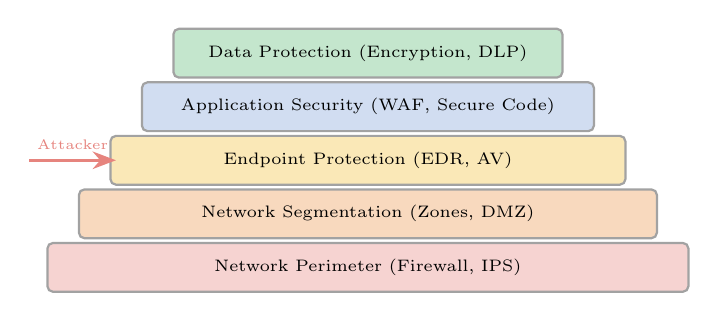
\begin{tikzpicture}[
  font=\fontsize{6.8pt}{8.5pt}\selectfont,
  >=Stealth
]
  %% Widths decrease inward to give a funnel / layered look
  \def\h{0.62}   %% row height
  \def\gap{0.06} %% vertical gap between rows

  %% Row definitions: {ypos}{width}{fill}{label}
  \foreach \yi/\wi/\col/\lbl in {
    0.00/8.0cm/cred!25/{Network Perimeter (Firewall, IPS)},
    0.68/7.2cm/corange!30/{Network Segmentation (Zones, DMZ)},
    1.36/6.4cm/cyellow!35/{Endpoint Protection (EDR, AV)},
    2.04/5.6cm/cblue!25/{Application Security (WAF, Secure Code)},
    2.72/4.8cm/cgreen!30/{Data Protection (Encryption, DLP)}
  }{
    \node[
      rectangle, rounded corners=2pt,
      minimum width=\wi, minimum height=\h cm,
      draw=cgray!60, thick, fill=\col,
      text centered, text width=\wi,
      font=\fontsize{6.5pt}{8pt}\selectfont,
      inner sep=2pt
    ] at (0,\yi) {\lbl};
  }

  %% Attacker arrow on the left
  \draw[-{Stealth}, thick, cred!70, line width=1.2pt]
    (-4.3, 1.36) -- (-3.2, 1.36)
    node[midway, above, font=\fontsize{5.5pt}{7pt}\selectfont,
         text=cred!70] {Attacker};

\end{tikzpicture}
\caption{Defense-in-depth layer stack. Each layer reduces residual risk passed to the
  next; no single failure results in full compromise.}
\label{fig:did}
\end{figure}

%%──────────────────────────────────────────────────────────────────────────────
\section{Decision Framework for Resilience}
%%──────────────────────────────────────────────────────────────────────────────

Cyber architects must weigh five factors when selecting resilience concepts.

\textbf{Mission Requirements.} Organizations supporting life-safety systems require
higher resilience than those with tolerance for brief outages~\cite{guidehouse2023}.

\textbf{Asset Sensitivity.} Systems handling Controlled Unclassified Information (CUI)
must meet CMMC requirements; the nature of protected data shapes control
priorities~\cite{dod2021cmmc}.

\textbf{Financial Resources.} Budget realities must be balanced against ideal resilience
architectures~\cite{metricstream2024,fortinet2024}.

\textbf{Organizational Maturity.} Technical workforce capability determines whether
advanced controls can be sustained; security orchestration platforms require skilled
analysts~\cite{guidehouse2023}.

\textbf{Threat Landscape.} Systems facing sophisticated adversaries require more rigorous
segmentation, monitoring, and identity protection~\cite{isaca2024}.

\begin{table}[h]
\caption{Resilience Concept Selection Criteria.}
\label{tab:selection}
\small
\begin{tabularx}{\columnwidth}{@{}p{2.4cm}X@{}}
\toprule
\textbf{Factor} & \textbf{Consideration} \\
\midrule
Mission Requirements  & Downtime tolerance, availability needs \\
\addlinespace[3pt]
Asset Sensitivity     & Data classification, CUI requirements \\
\addlinespace[3pt]
Financial Resources   & Budget constraints, TCO analysis \\
\addlinespace[3pt]
Org.\ Maturity        & Staffing skills, operational capacity \\
\addlinespace[3pt]
Threat Landscape      & Adversary sophistication, attack trends \\
\bottomrule
\end{tabularx}
\end{table}

%%──────────────────────────────────────────────────────────────────────────────
\section{Integration: Controls and Resilience}
%%──────────────────────────────────────────────────────────────────────────────

Compensating controls and cyber resilience strategies are complementary. Organizations
implementing compensating controls should embed them within broader resilience frameworks
under five guiding principles: (1)~\textit{Layered approach}---compensating controls
become elements of defense-in-depth strategies; (2)~\textit{Risk context}---both require
rigorous risk assessment and continuous monitoring; (3)~\textit{Operational reality}---
both acknowledge that perfect security is unattainable; (4)~\textit{Measurement}---both
demand measurable outcomes; and (5)~\textit{Evolution}---both require ongoing
reassessment as threats change.

The goal is achieving ``as secure as reasonably practicable'' (ASARP)---a standard
recognizing that organizations must balance security objectives against operational
requirements, cost constraints, and technical limitations~\cite{kelley2023,
guidehouse2023}.

%%
%% FIGURE 3 — Cyber Resilience Capability Wheel
%%
%% Design: four quadrant boxes arranged around a central label.
%% Box centres at (±1.45, ±1.0). Box width=2.5cm, height=1.5cm.
%% Max extent: 1.45 + 1.25 = 2.70 cm from centre on each side → 5.4 cm total  ✓
%%
\begin{figure}[h]
\centering
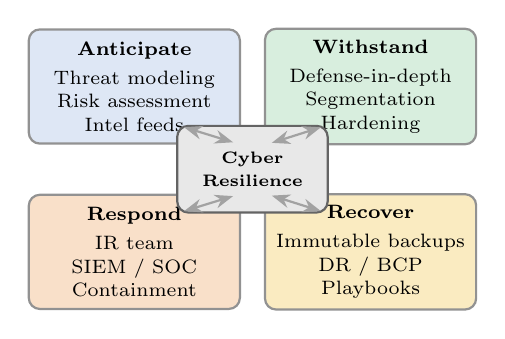
\begin{tikzpicture}[
  font=\fontsize{6.8pt}{8.5pt}\selectfont,
  >=Stealth,
  qbox/.style={
    rectangle, rounded corners=4pt,
    minimum width=2.55cm, minimum height=1.45cm,
    draw=cgray!70, thick,
    text centered, text width=2.4cm,
    align=center, inner sep=4pt
  },
  cbox/.style={
    rectangle, rounded corners=4pt,
    minimum width=1.8cm, minimum height=1.1cm,
    draw=cgray, thick, fill=cgray!15,
    text centered, text width=1.7cm,
    align=center, font=\fontsize{6.5pt}{8pt}\selectfont\bfseries,
    inner sep=3pt
  },
  arr/.style={<->, thick, cgray!60, shorten >=3pt, shorten <=3pt}
]

  %% ── Four quadrant boxes ──────────────────────────────────────────────────
  \node[qbox, fill=cblue!18]    (ant) at (-1.5, 1.05)
    {\textbf{Anticipate}\\[2pt]Threat modeling\\Risk assessment\\Intel feeds};

  \node[qbox, fill=cgreen!20]   (wit) at ( 1.5, 1.05)
    {\textbf{Withstand}\\[2pt]Defense-in-depth\\Segmentation\\Hardening};

  \node[qbox, fill=cyellow!30]  (rec) at ( 1.5,-1.05)
    {\textbf{Recover}\\[2pt]Immutable backups\\DR / BCP\\Playbooks};

  \node[qbox, fill=corange!25]  (res) at (-1.5,-1.05)
    {\textbf{Respond}\\[2pt]IR team\\SIEM / SOC\\Containment};

  %% ── Central label ────────────────────────────────────────────────────────
  \node[cbox] (ctr) at (0,0) {Cyber\\Resilience};

  %% ── Diagonal arrows between quadrants ────────────────────────────────────
  \draw[arr] (ant.south east) -- (ctr.north west);
  \draw[arr] (wit.south west) -- (ctr.north east);
  \draw[arr] (rec.north west) -- (ctr.south east);
  \draw[arr] (res.north east) -- (ctr.south west);

\end{tikzpicture}
\caption{The four pillars of cyber resilience: Anticipate, Withstand, Respond, and
  Recover, each feeding into the central resilience posture.}
\label{fig:resilience}
\end{figure}

%%──────────────────────────────────────────────────────────────────────────────
\section{Practical Recommendations}
%%──────────────────────────────────────────────────────────────────────────────

\subsection{For Compensating Controls}

Organizations should: establish formal processes for requesting, evaluating, and
approving compensating controls; require standardized documentation aligned with
regulatory frameworks; mandate risk assessments demonstrating equivalence; implement
annual review cycles; train auditors on evaluation criteria; maintain centralized
repositories tracking all approved controls; and create roadmaps for transitioning to
primary controls when feasible.

\subsection{For Cyber Resilience}

Organizations should: adopt the mindset that breaches are inevitable; implement
defense-in-depth across all system layers; prioritize network segmentation and
micro-segmentation; invest in detection and monitoring capabilities; test incident
response and recovery procedures regularly; maintain immutable backups with verified
restoration; conduct threat modeling identifying likely attack scenarios; integrate
resilience into system development lifecycles; and foster an organizational culture
where security is a shared responsibility.

%%──────────────────────────────────────────────────────────────────────────────
\section{Conclusion}
%%──────────────────────────────────────────────────────────────────────────────

Compensating controls represent essential mechanisms for maintaining security when ideal
solutions prove impractical. Rather than compliance shortcuts, properly designed
compensating controls are deliberate architectural decisions that provide equivalent risk
reduction through alternative means. The key to effective implementation lies in rigorous
justification, measurable outcomes, comprehensive documentation, and continuous
reassessment.

When integrated with broader cyber resilience strategies---including defense-in-depth,
network segmentation, identity governance, detection capabilities, and recovery
engineering---compensating controls enable organizations to maintain robust security
postures despite real-world constraints. Cyber resilience shifts focus from impossible
perfect prevention to realistic goals of withstanding attacks, detecting intrusions
rapidly, responding effectively, and recovering operations swiftly.

Organizations must recognize that resilience is not about eliminating all risks but about
building systems capable of enduring and recovering from inevitable adversity. This
requires abandoning checkbox compliance mindsets in favour of risk-based approaches that
acknowledge operational realities while maintaining defensible security postures. The
future of cybersecurity architecture lies in thoughtful adaptation that maintains
security objectives while respecting operational constraints---compensating controls and
cyber resilience strategies together provide the framework for this balanced, pragmatic
approach.

%%──────────────────────────────────────────────────────────────────────────────
\sloppy
\bibliographystyle{ACM-Reference-Format}
\begin{thebibliography}{99}

\bibitem{claroty2024}
Claroty. 2024. OT:ICEFALL Vulnerabilities Underscore the Importance of Compensating
Controls.
\url{https://claroty.com/blog/ot-icefall-vulnerabilities-underscore-the-importance-of-compensating-controls}

\bibitem{dod2021cmmc}
U.S. Department of Defense. 2021. \textit{Cybersecurity Maturity Model Certification
(CMMC) Model Version 2.0}. Chief Information Officer.

\bibitem{fortinet2024}
Fortinet. 2024. A Practical Guide to Designing and Applying Compensating Controls.
\url{https://www.fortinet.com/resources/cyberglossary/compensating-controls}

\bibitem{guidehouse2023}
Guidehouse. 2023. Building Resilience in Security Architecture.
\url{https://guidehouse.com/insights/advanced-solutions/2023/building-resilience-in-security-architecture}

\bibitem{ibm2024breach}
IBM Security. 2024. \textit{Cost of a Data Breach Report 2024}.

\bibitem{isaca2024}
L.~Marks. 2024. Cyber Resilience Through More Effective Design. \textit{ISACA Journal}.
\url{https://www.isaca.org/resources/news-and-trends/isaca-now-blog/2024/cyber-resilience-through-more-effective-design}

\bibitem{kelley2023}
D.~Kelley and E.~Moyle. 2023. \textit{Practical Cybersecurity Architecture}. Wiley.

\bibitem{koleyjessen2024}
Koley Jessen. 2024. Next Part of New York's Cybersecurity Regulation Takes Effect.
\url{https://www.koleyjessen.com/insights/publications/next-part-of-new-yorks-cybersecurity-regulation-takes-effect}

\bibitem{metricstream2024}
MetricStream. 2024. What is Compensating Controls?
\url{https://www.metricstream.com/learn/compensating-controls.html}

\bibitem{naruc2024}
NARUC and U.S. Department of Energy. 2024. \textit{Cybersecurity Baselines for Electric
Distribution Systems and DER}.
\url{https://pubs.naruc.org/pub/35247A70-0C45-9652-C6D9-99A77C87200F}

\bibitem{networkcomputing2024}
Network Computing. 2024. Structured for Success: 4 Architectural Pillars of Cyber
Resilience.
\url{https://www.networkcomputing.com/network-resilience/structured-for-success-4-architectural-pillars-of-cyber-resilience}

\bibitem{nist2020controls}
NIST. 2020. \textit{Security and Privacy Controls for Information Systems and
Organizations} (SP 800-53 Rev.\ 5). U.S. Department of Commerce.

\bibitem{nist2021resilience}
NIST. 2021. \textit{Developing Cyber-Resilient Systems} (SP 800-160 Vol.\ 2 Rev.\ 1).
U.S. Department of Commerce.

\bibitem{nistglossary2024}
NIST. 2024. Compensating Security Control. \textit{CSRC Glossary}.
\url{https://csrc.nist.gov/glossary/term/compensating_security_control}

\bibitem{reach2024}
Reach Security. 2024. Compensating Controls: The Unsung Heroes of Cyber Resilience.
\url{https://www.reach.security/blog/compensating-controls-the-unsung-heroes-of-cyber-resilience}

\bibitem{rockwell2024}
Rockwell Automation. 2024. Compensating Controls in OT Security.
\url{https://www.rockwellautomation.com/en-us/company/news/blogs/compensating-control-ot.html}

\bibitem{specops2022}
Specops Software. 2022. Understanding Compensating Controls and How to Use Them.
\url{https://specopssoft.com/blog/compensating-security-controls/}

\bibitem{techtarget2024}
TechTarget. 2024. What is a compensating control and how is it implemented?
\url{https://www.techtarget.com/searchsecurity/definition/compensating-control}

\bibitem{zeronetworks2024}
Zero Networks. 2024. Cyber Resilience Architecture: Key Strategies for Effective
Protection.
\url{https://zeronetworks.com/blog/cyber-resilience-architecture/}

\end{thebibliography}

\end{document}
